\documentclass[10pt,letter]{article}
	% basic article document class
	% use percent signs to make comments to yourself -- they will not show up.

\usepackage{amsmath}
\usepackage{amssymb}
	% packages that allow mathematical formatting

\usepackage{graphicx}
	% package that allows you to include graphics

\usepackage{setspace}
	% package that allows you to change spacing

\onehalfspacing
	% text become 1.5 spaced

\usepackage{fullpage}
	% package that specifies normal margins
	
\usepackage[version=3]{mhchem} % Package for chemical equation typesetting
\usepackage{graphicx} % Required for the inclusion of images
\usepackage{natbib} % Required to change bibliography style to APA
\usepackage{amsmath} % Required for some math elements 
\usepackage{booktabs}
\usepackage{floatrow}
	

\begin{document}
	% line of code telling latex that your document is beginning


\title{CS 156 Problem Set 6}

\author{Christopher Zhen}

\date{Nov 7, 2016}
	% Note: when you omit this command, the current dateis automatically included
 
\maketitle 
	% tells latex to follow your header (e.g., title, author) commands.
	
\section*{Problem 1}

\textbf{(B)} - Since we're trying to fit the same function with a smaller hypothesis set, our hypothesis generally won't fit as well, so there will be an increase in deterministic noise.

\section*{Problem 2}

\textbf{(A)} - According to our code, our in sample error is 0.028 and our out of sample error is 0.084 which is closest to answer A.

%\begin{figure}[H]
%\begin{center}
%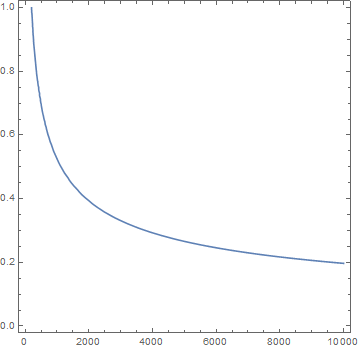
\includegraphics[width=0.5\textwidth]{2d.png}
%\caption{Table courtesy of the textbook %textit{Learning from Data}.}
%\label{2d}
%\end{center}
%\end{figure}

\section*{Problem 3} 

\textbf{(D)} - Our code ouputs errors similar to before (0.029 and 0.08) because lambda is very small and doesn't make much of a difference.

\section*{Problem 4}

\textbf{(E)} - This time we get huge errors (0.37 and 0.44) due to the large lambda.

\section*{Problem 5}

\textbf{(D)} - Even though $k = 0$ gives you the best in-sample error (error = 0), the best out-of-sample error is attained when $k = -1$ with an out-of-sample error of $0.056$.

\section*{Problem 6}

\textbf{(B)} - The code outputs an error of $0.056$ which is closest to answer choice B when using $k=-1$. Something interesting to note is that if we didn't have the out-of-sample points, we would've chosen $k=0$ which would've given us an out-of-sample error of $0.092$ which is significantly worse.

\section*{Problem 7}

\textbf{(C)} - In answer choice C, $\mathcal{H}(10, 0, 3)$ is equivalent to $\mathcal{H}_2$ and $\mathcal{H}(10,0,4)$ is equivalent to $\mathcal{H}_3$. The intersection of $\mathcal{H}_2$ and $\mathcal{H}_3$ is simply $\mathcal{H}_2$, so answer choice C is correct.

\section*{Problem 8}

\textbf{(D)} - First we need to compute the gradient which is done by summing all the $w_{ij}^{(l)}x_i^{(l-1)}$ terms. This comes out to be $6 * 3 + 4* 1 = 22$. Next we need to compute all the required $\delta _j^{(l)}$ values. Since we only need these partials for three nodes in the middle layer (since we already know it for the output node and we don't need it for $x_0^{(1)}$), we only need $1*3 = 3$ computations to find all the $\delta _j^{(l)}$ values. Finally, we need to update the weights which is done by multiplying all the $w_{ij}^{(l)}$ by the corresponding $\delta _j^{(l)}$ terms. This number also comes out to 22 since each $w_{ij}^{(l)}$ maps to a single $\delta _j^{(l)}$, so we just count the $w_{ij}^{(l)}$ terms again. Summing up we get $22 + 3 + 22 = 47$ which is closest to answer choice D.

\section*{Problem 9}

\textbf{(A)} - The neural network with the least amount of weights involves the least number of nodes in each layer (2) to minimize multiplicative terms. This gives us 10 weights going into the first hidden layer and then 36 weights until the output node; or 46 total weights.

\section*{Problem 10}

\textbf{(E)} - In this case we want to have 2 hidden layers because having more hidden layers just adds more terms at the cost of multiplying more terms which would give us fewer weights. With two hidden layers, we have the following expression that we need to maximize (where x is the number of nodes in the first hidden layer):

\begin{equation}
10(x-1) + x(35-x) + 36-x
\end{equation}

This expression is maximized when $x = 22$ with the value 510 which matches answer choice E.

\end{document}
	% line of code telling latex that your document is ending. If you leave this out, you'll get an error
